\section{Supplementary Numerical Results}\label{app: supp-numerical}
\subsection{Numerical optimization of $\m{0}$ in 1D}
To test whether numerical optimization is a practical way to solve \eqref{eq: bi-orth-eq}, we first experiment on $m_0(\omega)$ and $\m{0}$ of pre-designed bi-orthogonal wavelets. We consider a low frequency filters corresponding to bi-orthogonal scaling functions $\phi,\, \tilde{\phi}$ with vanishing moments 3 and 5 respectively. 

\begin{wrapfigure}{r}{.4\textwidth}
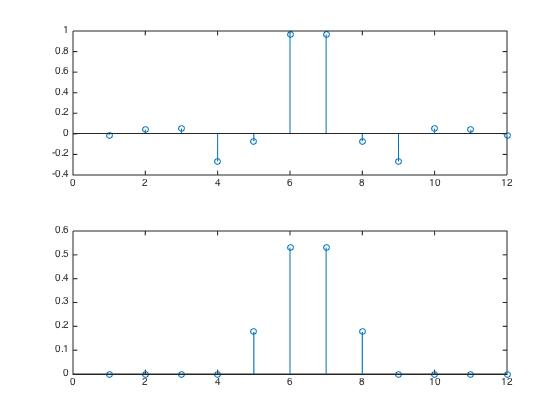
\includegraphics[width = .4\textwidth]{filters.jpg}
\caption{1d filters, up: LoD, down: LoR}
\label{fig: filters}
\end{wrapfigure}
The filters are shown in Fig.\ref{fig: filters}. Suppose we know the upper decomposition filter, and we want to find the lower reconstruction filter by solving \eqref{eq: bi-orth-eq}, such that the filter has support as compact as possible. The corresponding $m_0$ and $\widetilde{m_0}$ are complex, yet we can shift the phase of $m_0$ such that $m_0$ is real and apply the same phase shift to $\m{0}$. Without loss of generality, \eqref{eq: bi-orth-eq} can be solved assuming that $m_0$ is  real.
It is not necessary that the corredponding $\widetilde{m_0}$ is also real, but in this testing case, $m_0(\V{\omega})$ and $\m{0}$ have the same phase, hence the phase-shifted $\m{0}$ is real as well. Fig.\ref{fig: m-funcs} shows the ground truth $m_0(\V{\omega})$ and $\m{0}$ considered in this simulation. %and in particular, $|m_0|$ is used as the known coefficients in \eqref{eq: bi-orth-eq}. Hereafter, we use $m_0(\omega)$ and $\m{0}$ to denote the real-valued functions.
\begin{figure}%{l}{.4\textwidth}
\begin{minipage}{.5\textwidth}
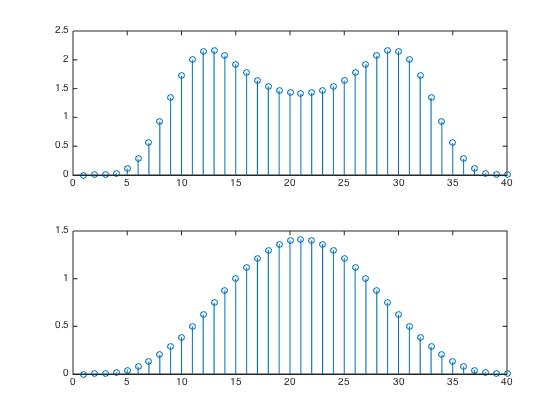
\includegraphics[width = \linewidth]{m-funcs.jpg}
\caption{$m_0(\V{\omega})$ and $\m{0}$}
\label{fig: m-funcs}
\end{minipage}
\hfill
\begin{minipage}{.4\textwidth}
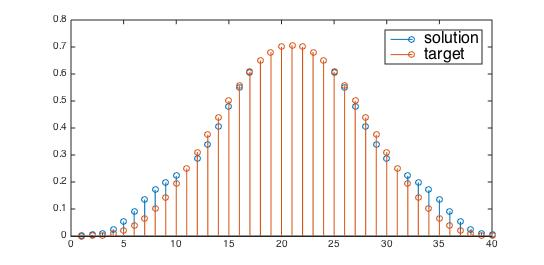
\includegraphics[width = \textwidth]{1d-m-compare.jpg}\\
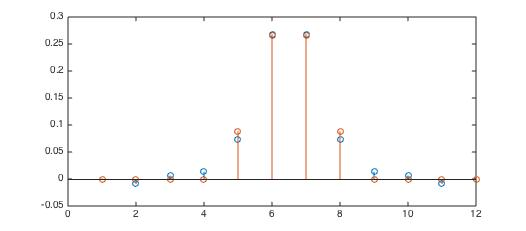
\includegraphics[width = \textwidth]{1d-filter-compare.jpg}
\caption{$\mhat{0}$ vs. $\m{0}$}
\label{fig: 1d-compare}
\end{minipage}
\end{figure}

Let $\mhat{0}$ be the approximation of $\m{0}$, which is solution of the following optimization problem
\begin{align}
\min_{\xvec}\; \Vert \V{D}\xvec\Vert^2 + \Vert \xvec\Vert^2,\quad s.t. \; \V{A}\xvec = \mathbf{1} \label{eq: opt-1d}
\end{align}
where $\V{A}$ in the constraint is the matrix generated from \eqref{eq: identity-cond} (in 1D, only a single shift of $\pi$ appears in the condition, so each row of $\V{A}$ has two non-zero entries). Notice that no symmetry constraint is imposed here, nevertheless, the solution shown in Fig.\ref{fig: 1d-compare} is almost symmetric. On the other hand, its support in the time domain is not as compact as that of $\m{0}$, see the bottom of Fig.\ref{fig: 1d-compare}.

\subsection{Numerical optimization of $\m{0}$ in 2D}
\begin{minipage}[c]{.45\textwidth}
\centering
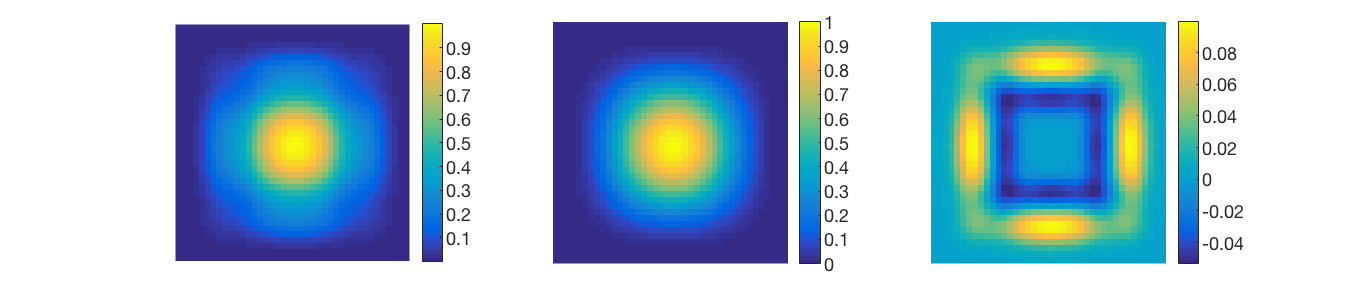
\includegraphics[width = \textwidth]{2d-m-compare-vanilla.png}
\captionof{figure}{Left: result of \eqref{eq: opt-1d} in 2D, Right: target}
\label{fig: 2d-compare-1}
\end{minipage}
\hfill
\begin{minipage}[c]{.5\textwidth}
The 2D case is much harder and several different optimization problems are formulated and their solutions are shown in the following. The 2D bi-orthogonal low-pass filters used here are the tensor products of the 1D filters used above.
{\it 2D version of \eqref{eq: opt-1d}}\\
 The 1D formulation can be easily extended to 2D, where $\V{D} = [\V{D}_x,\V{D}_y]$ consider 1st order derivative in both $x$ and $y$ directions, and $\V{A}$ is generated from \eqref{eq: identity-cond}, each row has four non-zero entries. Fig.\ref{fig: 2d-compare-1} shows the minimizer and compares it with the target function. It is obvious that the solution is not $90^\circ$-rotation invariant. Even worse is the fact that there is much energy in the vertical high-frequency domain.
\end{minipage}
\\[1em]
%{\it weighted L2 norm (Modulation Space$^{[\ref{app: modulation}]}$)}\\
To enforce the support of $\mhat{0}$ concentrates within the low frequency domain, the squared $\ell_2$-norm regulator in \eqref{eq: opt-1d} is changed to a weighted version (corresponding to Modulation space) as follows,
\begin{align}
\min_{\xvec}\; \Vert\V{ D}\xvec\Vert^2 + \lambda\Vert \wvec\circ\xvec\Vert^2,\quad s.t. \; \V{A}\xvec = \mathbf{1} \label{eq: opt-2d-weight}
\end{align} 
where $\circ$ is Hadamard product and $\wvec$ is a weight vector. In particular, we choose $\forall \omega, \; \wvec(\V{\omega}) = \Vert\V{\omega}\Vert$. Fig.\ref{fig: 2d-compare-2} and Fig.\ref{fig: 2d-compare-2.2} show the minimizer of \eqref{eq: opt-2d-weight} with $\lambda=60$ and $600$ respectively. As $\lambda$ increases, the support of the minimizer concentrates more within the low frequency region. As shown in Fig.\ref{fig: 2d-compare-2}, when $\lambda$ is not huge, the minimizer achieves a certain level of but not full symmetry, whereas Fig.\ref{fig: 2d-compare-2.2} shows that huge $\lambda$ imposes full symmetry.

\begin{comment}
\begin{minipage}{.9\textwidth}
\centering
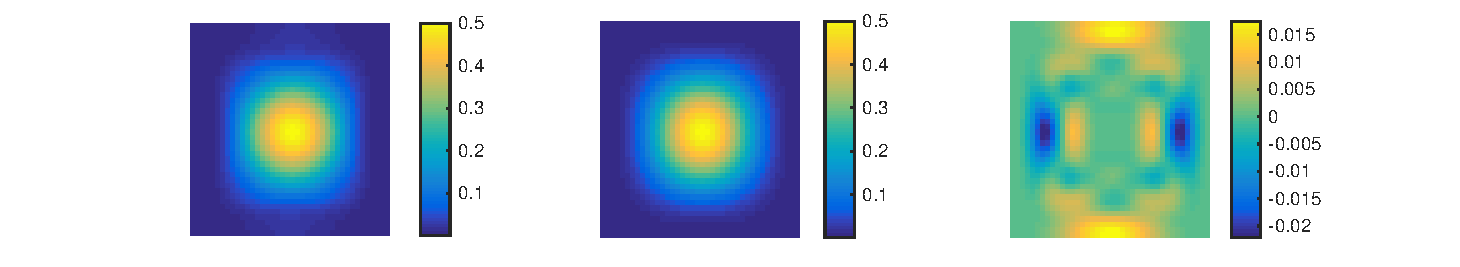
\includegraphics[width = .9\textwidth]{2d-m-compare-2-1-eps-converted-to.pdf}\\
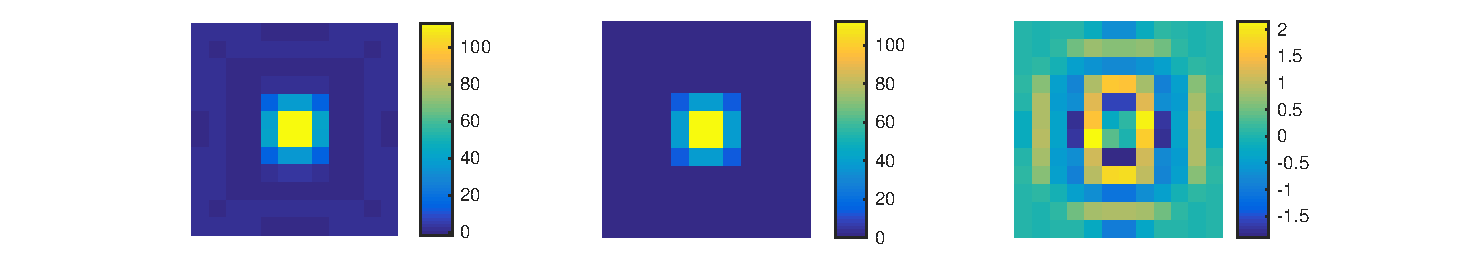
\includegraphics[width = .9\textwidth]{2d-filter-compare-2-1-eps-converted-to.pdf}
\captionof{figure}{result of \eqref{eq: opt-2d-weight} $\mhat{0}$ ($\lambda = 60$), target $\m{0}$ and their difference, Top: frequency domain, Bottom: time domain}
\label{fig: 2d-compare-2}
\end{minipage}
\end{comment}
\vspace*{2em}
\begin{minipage}{.9\textwidth}
\centering
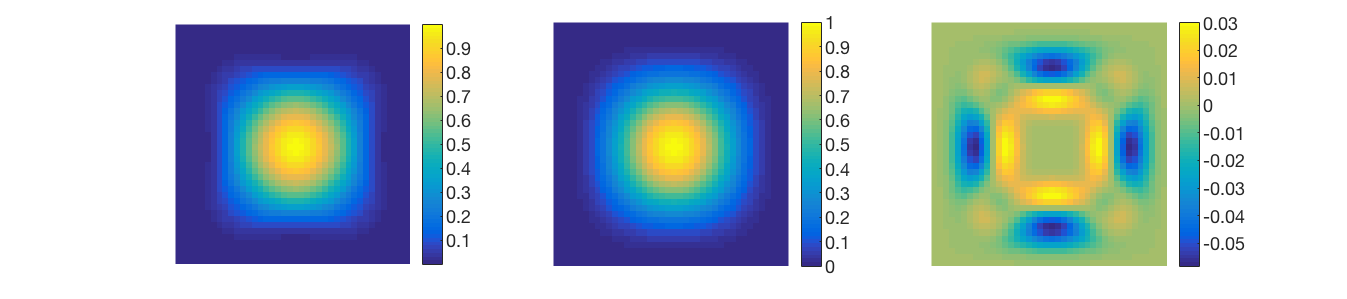
\includegraphics[width = .9\textwidth]{2d-m-compare-weightedl2.png}\\
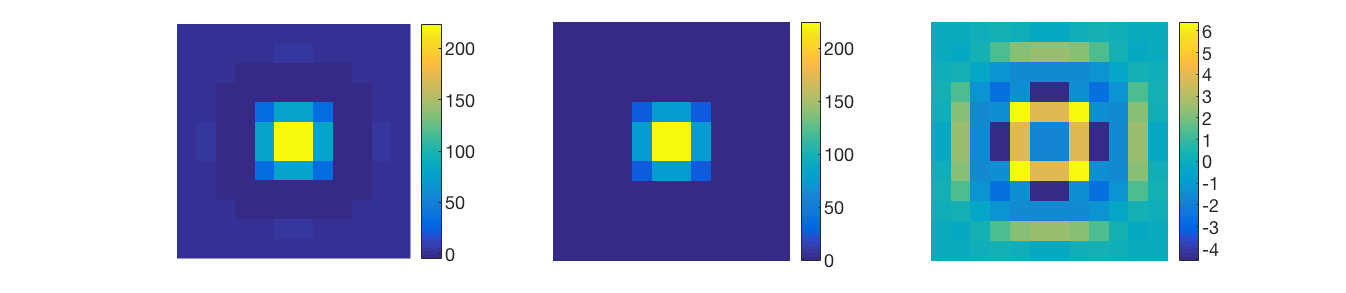
\includegraphics[width = .9\textwidth]{2d-filter-compare-weightedl2.png}
\captionof{figure}{result of \eqref{eq: opt-2d-weight} $\mhat{0}$ ($\lambda = 600$), target $\m{0}$ and their difference}
\label{fig: 2d-compare-2.2}
\end{minipage}
\\[1em]
{\it weighted L2 norm with symmetry constraint}\\
If we hard constrain the symmetry by the following
\begin{align}
\min_{\xvec}\; \Vert \V{D}\xvec\Vert^2 + \lambda\Vert \wvec\circ\xvec\Vert^2,\quad s.t. \; \V{A}\xvec = \mathbf{1},\,\V{S}\xvec = \mathbf{0} \label{eq: opt-2d-weight-sym}
\end{align}
where each row of $\V{S}$ has an one entry and a negative one entry at the location of two points have the same value due to symmetry. In practice, we put symmetry constraints such that the upper half plane is symmetric to the lower half plane w.r.t. $x$ coordinate and the first quadrant is $90^{\circ}-$ rotational invariant w.r.t. the second quadrant. The symmetry constraint makes the optimization problem significantly harder, resulting in longer optimization algorithm running time and no near-optimal solution is found (the algorithm terminates as the maximum number of iterations is exceeded). Fig.\ref{fig: 2d-compare-3} shows the result provided by the Matlab quadratic minimization solver, unfortunately, there are artifacts at the near endpoints of $x$ and $y$ coordinates.
\begin{figure}[h]
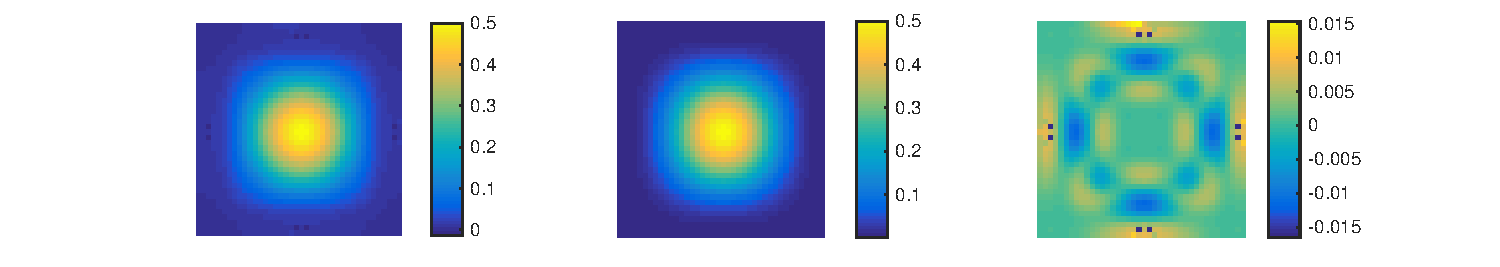
\includegraphics[width = .9\textwidth]{2d-m-compare-3-eps-converted-to.pdf}\\
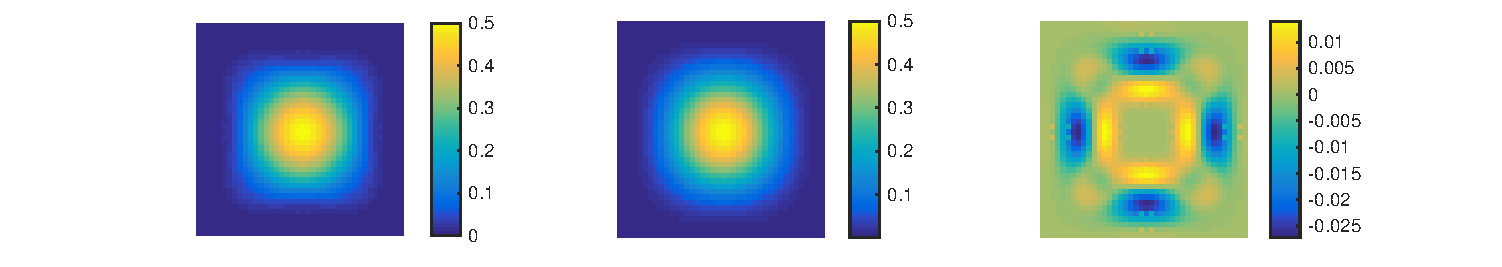
\includegraphics[width = .9\textwidth]{2d-m-compare-3-2-eps-converted-to.pdf}
\caption{solution of \eqref{eq: opt-2d-weight-sym} (top: $\lambda=60$, bottom: $\lambda=600$) provided by Matlab solver \texttt{quadprog}}
\label{fig: 2d-compare-3}
\end{figure}
\\
On the other hand, asymmetric solution can always be symmetrized by the average of the solution and its dual
w.r.t. rotation, mirroring, etc. This approach increase the support of the solution, thus a well concentrated solution in the frequency domain is necessary to begin with.
\\[1em]
{\it Other potential formulations}\\
We may also putting weights in the first L2-norm of derivatives, such that
\begin{align}
\min_{\xvec}\; \Vert \wvec'\circ \V{D}\xvec\Vert^2 + \lambda\Vert \wvec\circ\xvec\Vert^2,\quad s.t. \; \V{A}\xvec = \mathbf{1} \label{eq: opt-2d-double-weight}
\end{align}
Clearly, $\wvec'(\V{\omega})\rightarrow +\infty$ as $|\V{\omega}|\rightarrow +\infty$, but its behavior near the origin is unclear.